\documentclass[10pt]{article}
\usepackage{mathtools}
\usepackage{graphicx}
\usepackage{amsmath}
\usepackage{amsfonts}
\usepackage{microtype}
\usepackage{hyperref}
\usepackage{tikz-cd}
\usepackage{amssymb}
\usepackage{comment}
\usepackage{mymacros}
\usepackage{caption}
\usepackage{subcaption}
\usepackage{biblatex}

\addbibresource{refrences.bib}

\setlength{\parindent}{0cm} 
\setlength{\parskip}{1em}

\graphicspath{{./img/}}

\begin{document}
\begin{center}
  \large \textbf{Solving the 1D-Poisson Equation Numerically}

  \text{Kristian Gjestad Vangsnes}
  
  \textit{Department of physics, University of Oslo}


  \text{Date: 9. September 2019}
\end{center}
\begin{abstract}
  abstract 


\end{abstract}
\section{Introduction}
In this project we will study numerical algorithm which solves the differential equation Poisson's equation, this is the equation which modulates the change of a electric potential. 

Two algorithms will be based on Gaussian-elimination and is programed on a lower level using c++, while the third algorithm is the famous LU-decomposition and will be computed using the linear algebra library Armadillo.

The focus of this report is to compare the efficiency and precision of the algorithms.

\section{Theory}
The one-dimentional Poisson equation 
with Dirichlet boundary conditions reads 

\begin{equation*}
 -u''(x)=f(x),\quad x\in (0,1),\quad u(0)=u(1)=0.
\end{equation*}

We will use the source term $f(x)=100e^{-10x}$. This gives the particular solution 
$u(x)=1-(1-e^{-10})x-e^{-10x}$. We will compare our numerical solution to this exact solution.

We will also compute the relative error for our algorithms. The relative error is defined as 
$$ \epsilon=\log{\left|\frac{u_{numerical}-u_{exact}}{u_{exact}}\right|}.$$

\section{Numerical methods}
In order to model this equation in a computer we need to define the 
discretized approximated solution to $ u(x) $ as $v_i=v(x_i) $ where
 $x_i=x_0+ih=ih$ since $x_0=0$. We let $x_{n+1}=1$, this means $h=\frac{1}{n+1}$.
 From Taylor expanding $u(x\pm h)$ we get 
 $$u(x\pm h)=u(x)\pm hu'(x)+\frac{h^2}{2!}u''(x)\pm O(h^3)$$
We see that $u''(x)=\frac{u(x+h)+u(x-h)-2u(x)}{h^2}-O(h^4)$. Hence for the approximated solution
 we get that $$-\frac{v_{i+1}+v_{i-1}-2v_i}{h^2}=f_i\quad \text{for i}=1,...,n$$ where $f_i=f(x_i)$. 
 If we set $g_i=h^2f_i$ we get that $2v_i-v_{i+1}-v_{i-1}=g_i$. 
 This is just $n$ equations, given by $i=i,...,n$. We can write this in matrix form 
 $$\mathbf{A}\mathbf{v}=\mathbf{g}, $$ where $\mathbf{A}$ is a $n\times n$ 
 tridiagonal matrix on the form $$\mathbf{A}=\begin{bmatrix}
   2 & -1 & 0 & \dots & ... & 0 \\
   -1 & 2 & -1 & 0 & ... & 0 \\
   0  & -1 & 2 & -1 & 0 & ... \\
   \vdots & 0 & \ddots & \ddots & \ddots & ...\\
   0 & ... & ... & -1 & 2 & -1\\
   0 & ... & ... & 0 & -1 & 2 
 \end{bmatrix}$$

 $\mathbf{v}$ and $\mathbf{g}$ are vectors on the form 
 $$\mathbf{v}=\begin{bmatrix}
   v_1\\v_2\\\vdots\\v_n
 \end{bmatrix}
 \qquad
 \mathbf{g}=\begin{bmatrix}
   g_1\\g_2\\\vdots\\g_n
 \end{bmatrix}
 $$

 The relative error is computed by $$ \epsilon=\log{\left|\frac{v_{i}-u_{i}}{u_{i}}\right|}.$$


 \subsection{General algorithm}
 The general algorithm to solve a set of equation on a tridiagonal form is done by Gaussian elimination, and is called the Thomas algorithm \cite{thomas}.  The algorithm On matrix form the problem is $\mathbf{A}\mathbf{v}=\mathbf{g}$. Where $\mathbf{v}$ contains the unknowns $v_i$. In our case the unknowns are the solution to the Poisson equation at $x_i=ih$, i.e. $v(x_i)=v_i$.
 $$
 \mathbf{A}=  \begin{bmatrix}
  d_1 & b_1 & 0 & \dots & ... & 0 \\
  a_1 &d_2 & b_2 & 0 & ... & 0 \\
  0  & a_2 & d_3 & b_3 & 0 & ... \\
  \vdots & 0 & \ddots & \ddots & \ddots & ...\\
  0 & ... & ... & a_{n-2} & d_{n-1} & b_{n-1}\\
  0 & ... & ... & 0 & a_{n-1} & d_{n} 
 \end{bmatrix}, \qquad \mathbf{g}=\begin{bmatrix}
  g_1 \\ g_2 \\ \vdots \\ g_n
 \end{bmatrix}.
 $$
We see that the two first equations are 
\begin{equation}
  d_1v_1+b_1v_2=g_1
  \label{eq:eq1}
\end{equation}
\begin{equation}
  a_1v_1+d_2v_2+b_2d_3=g_2
  \label{eq:eq2}
\end{equation}

We see that if we multiply eq (\ref{eq:eq1}) by $\frac{a_1}{d_1}$ and subtract it from eq(\ref{eq:eq2}) we see that eq(\ref{eq:eq2}) becomes $$ (d_2-\frac{a_1b_1}{d_1})=g_2-\frac{a_1g_1}{d_1} $$. 

This is called forward substitution and generally for a tridiagonal matrix gives us the new diagonal elements 
$$\tilde{d}_{i+1}=d_{i+1}-\frac{a_ib_i}{\tilde{d_i}}$$  $$\tilde{g}_{i+1}=g_{i+1}-\frac{a_i\tilde{g_i}}{\tilde{d_i}}$$ Where $\tilde{d_1}=d_1$ and $\tilde{g}_1=g_1$. Now our problem in on the form $\mathbf{\tilde{A}}\mathbf{v}=\mathbf{\tilde{g}}$ where $$
\mathbf{\tilde{A}}=  \begin{bmatrix}
 \tilde{d}_1 & b_1 & 0 & \dots & ... & 0 \\
 0 &\tilde{d}_2 & b_2 & 0 & ... & 0 \\
 0  & 0 & \tilde{d}_3 & b_3 & 0 & ... \\
 \vdots & 0 & \ddots & \ddots & \ddots & ...\\
 0 & ... & ... & 0 & \tilde{d}_{n-1} & b_{n-1}\\
 0 & ... & ... & 0 & 0 & \tilde{d}_{n} 
\end{bmatrix}, \qquad \mathbf{g}=\begin{bmatrix}
 \tilde{g}_1 \\ \tilde{g}_2 \\ \vdots \\ \tilde{g}_n
\end{bmatrix}.
$$
To get the problem to a diagonal form we have to perform a backward substitution, this is done component wise by 
$$v_{n-i}=\frac{\tilde{g}_{n-i}-b_{n-i}v_{n+1-i}}{\tilde{d}_{n-i}}$$ where $v_{n}=\frac{\tilde{g}_n}{\tilde{d}_n}$. 

When we start to count from 0 to $n-1$ the algorithm goes as follows:

\begin{center}
  \begin{tabular}{||c||}
    \hline\hline
    \textbf{General Algorithm}\\
    \hline\hline
    Forward substitution \\
    \textbf{for} $i=0,1,2,...,n-1$\\
      $d_{i+1}-=a_i*b_i/d_i$ \\
      $g_{i+1}-=a_ig_i/d_i$ \\
      \textbf{End loop} \\
      Backward substitution \\
      $v_{n-1}=g_{n-1}/d_{n-1}$\\
      \textbf{for i=2, 3, ..., n} \\
      $v_{n-i}=(g_{n-i}-b_{n-i}v_{n+1-i})/d_{n-i}$\\ 
      \textbf{End loop}\\
      \hline\hline
  \end{tabular}
\end{center}
The number of floating points operations (FLOPS) performed in this general algorithm is $9n$, $6n$ FLOPS in the forward substitution, $2n$ subtractions, $2n$ multiplications and $2n$ divisions. $3n$ FLOPS in the backward substitution, $n$ subtraction, $n$ multiplication and $n$ division.


\subsection{Specialized algorithm}
When all the diagonal elements are equal and the off diagonal elements are equal we can make our algorithm more efficient. If we us the matrix $\mathbf{A}$ for the Poisson equation, we get a even more specialized algorithm. For equal diagonal elements and equal off diagonal elements we get the following algorithm.


\begin{center}
  \begin{tabular}{||c||}
    \hline\hline
    \textbf{Specialized Algorithm for equal diagonal and off diagonal terms}\\
    \hline\hline
    Diagonal term is $d$ and off diagonal term is $a$.\\
    $d_0=d$\\
    Let $A=a^2$, we precalculate in order to save memory.\\
    Forward substitution \\
    \textbf{for} $i=0,1,2,...,n-1$\\
      $d_{i+1}-=A/d_i$ Note \\
      $g_{i+1}-=a\times g_i/d_i$ \\
      \textbf{End loop} \\
      $v_{n-1}=g_{n-1}/d_{n-1}$\\
      Backward substitution \\
      \textbf{for i=2, 3, ..., n} \\
      $v_{n-i}=(g_{n-i}-a\times v_{n+1-i})/d_{n-i}$\\ 
      \textbf{End loop}\\
      \hline\hline
  \end{tabular}
\end{center}

This algorithm does $8n$ FLOPS, it does $5n$ FLOPS in the forward substitution, $2n$ subtractions, $2n$ divisions and $n$ multiplications. In the backward substitution we have $3n$ FLOPS, $n$ subtractions, $n$ multiplications and $n$ divisions.

But we can make a even better algorithm if the diagonal elements are $2$ and the off diagonal elements are $-1$. If that is the case we can use the following algorithm.

\begin{center}
  \begin{tabular}{||c||}
    \hline\hline
    \textbf{Specialized Algorithm for the Poisson problem}\\
    \hline\hline Note tha
    t the diagonal elemets are precalculated\\
    Forward substitution \\
    \textbf{for} $i=0,1,2,...,n-1$\\
      $g_{i+1}+=g_i/d_i$\\
      \textbf{End loop} \\
      Backward substitution \\
      $v_{n-1}=g_{n-1}/d_{n-1}$\\
      \textbf{for i=2, 3, ..., n} \\
      $v_{n-i}=(g_{n-i}+v_{n+1-i})/d_{n-i}$\\ 
      \textbf{End loop}\\
      \hline\hline
  \end{tabular}
\end{center}
 We see that since we have precalculated the diagonal elements and used that the off diagonal element is -1, the number of FLOPS is only $4n$.



\section{Program structure}



\section{results}

The general algorithm was programed using c++ and the solution for matrix size n=10, 100 and 1000 was compared to the exact solution and plotted using python as shown below.

  \begin{figure}[h]
    \centering 
    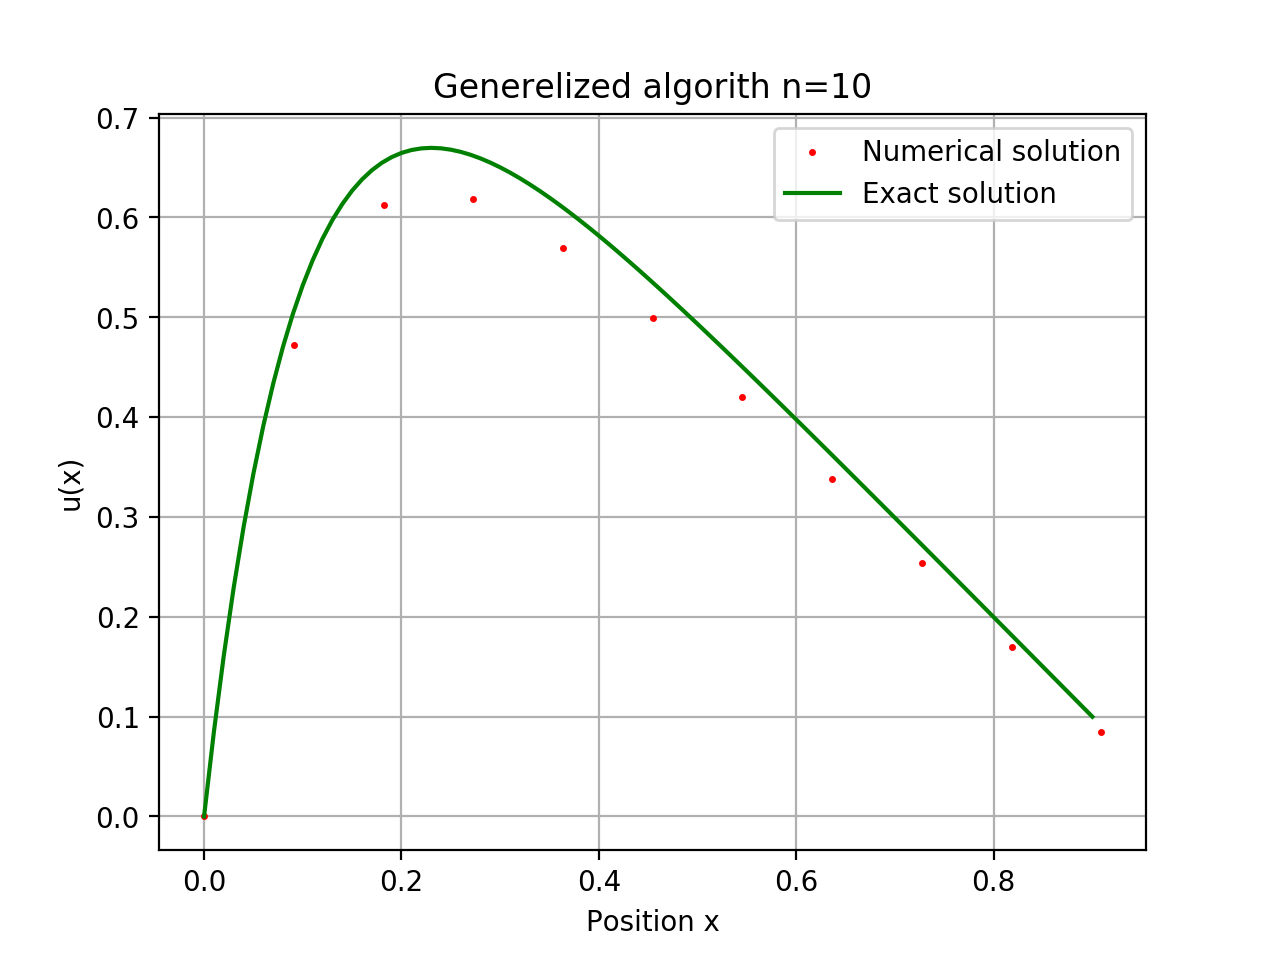
\includegraphics[scale=0.7]{alg-0-n10plot.png}
  \end{figure}
  \begin{figure}
    \centering
    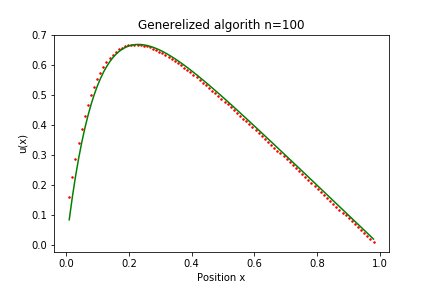
\includegraphics[scale=0.7]{alg-0-n100plot.png}
  \end{figure}
  \begin{figure}
    \centering
    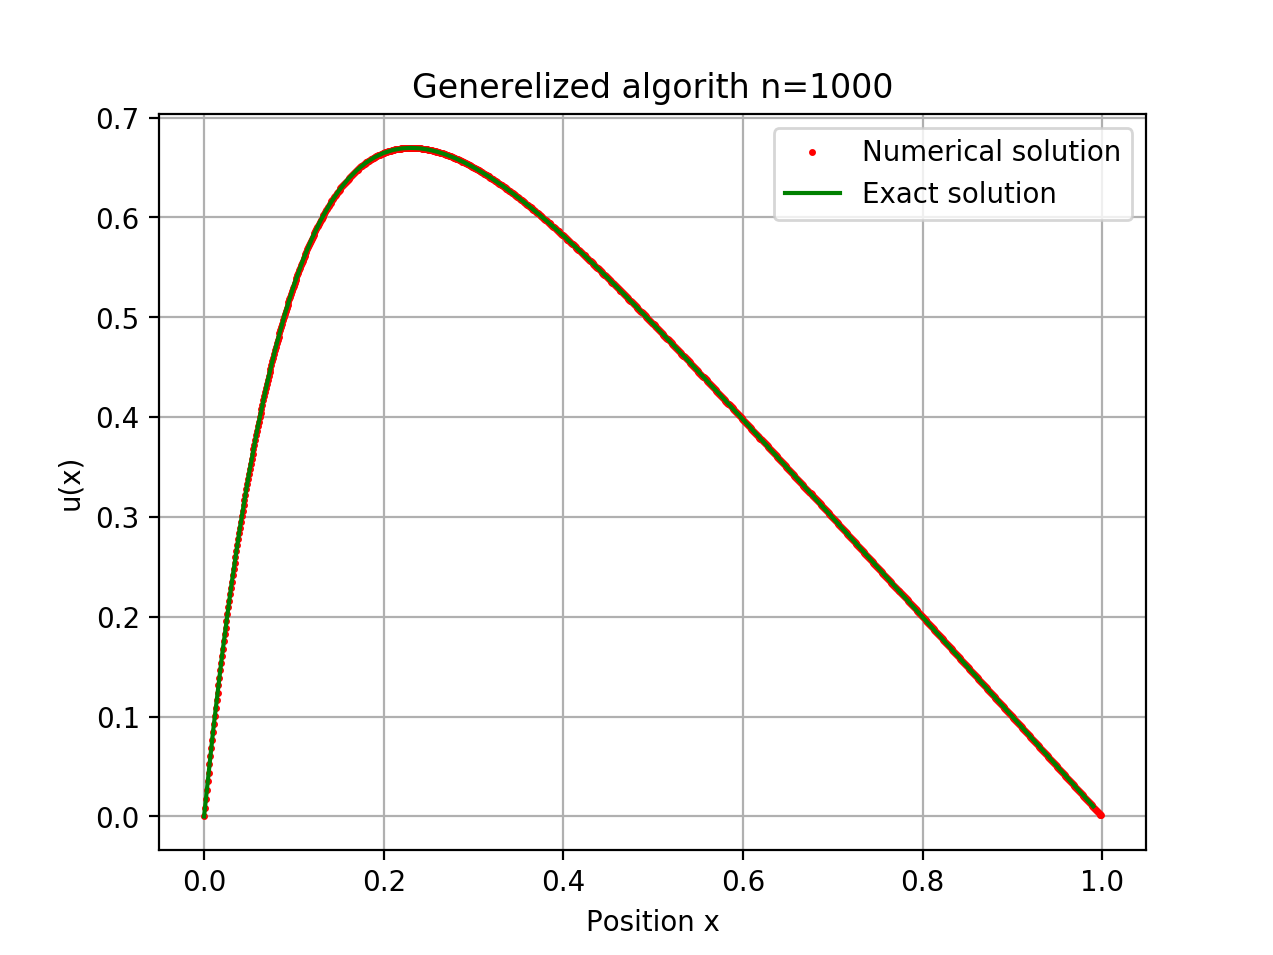
\includegraphics[scale=0.7]{alg-0-n1000plot.png}
  \end{figure}


We see that for the general solution $n=10$ is a bad approximation, this is because the step length is too long, i.e. too few grid points, which makes the approximation of the second derivative bad.

\section{Summary}

\printbibliography

\end{document}

